\documentclass[11pt]{article}

\usepackage[utf8]{inputenc}
\usepackage[T1]{fontenc}
\usepackage{lmodern}
\usepackage[margin=1in]{geometry}
\usepackage{amsmath,amssymb,amsthm}
\usepackage{booktabs}
\usepackage{graphicx}
\usepackage{microtype}
\usepackage[numbers,sort&compress]{natbib}
\usepackage[hidelinks]{hyperref}

\newtheorem{remark}{Remark}

% ---------------------------------------------------------------------------
% Result numbers, transcribed from results/report/results.json (seed 20231015).
% Update these macros when the results file changes; the tables read them.
% ---------------------------------------------------------------------------
\newcommand{\paretoStdIters}{40}
\newcommand{\paretoStdCuts}{195}
\newcommand{\paretoParIters}{27}
\newcommand{\paretoParCuts}{127}

\title{A Two-Stage Stochastic Capacitated Facility Location Solver with a
Service-Level Chance Constraint and Benders Decomposition:
Implementation and Computational Study}

\author{Mohammad S.\ Hajibabaie}
\date{}

\begin{document}
\maketitle

\begin{abstract}
We present an open, reproducible solver for the two-stage stochastic capacitated
facility location problem (CFLP) with a joint service-level chance constraint.
Facilities are opened in a first stage; under uncertain demand the recourse stage
serves customers and pays a penalty for unmet demand. The model is formulated as a
sample-average-approximation (SAA) mixed-integer program and solved either as a
monolithic extensive form or by an L-shaped Benders decomposition. Because the
recourse is relatively complete, the decomposition uses optimality cuts only; we
additionally implement Magnanti--Wong/Papadakos Pareto-optimal cuts. A single
cut-separation routine is shared by three interchangeable backends: an iterative
loop on HiGHS, a single-tree branch-and-Benders-cut on SCIP through a constraint
handler, and a single-tree implementation on Gurobi using lazy-constraint
callbacks. We validate correctness against the published optima of the OR-Library
\texttt{cap} instances and against the SAA monolith, quantify the value of the
stochastic solution (VSS) and the expected value of perfect information (EVPI) on
instances built from real city data, and report the effect of demand volatility
and of the chance-constraint risk level. We discuss the practical scaling limit
imposed by a plain-Python cut routine and outline the path to larger instances.
\end{abstract}

\section{Introduction}
\label{sec:intro}

Facility location under demand uncertainty is a canonical problem in operations
research and supply-chain design: a decision maker commits to opening facilities
before demand is known, and then serves realized demand at minimum cost
\citep{santoso2005,birge2011}. Two features make the problem both practically
relevant and computationally demanding. First, the first-stage decisions are
binary and the second-stage recourse is a continuous transportation problem, so
the deterministic equivalent is a large mixed-integer program. Second, a decision
maker often cares not only about expected cost but also about a \emph{service
level}: the guarantee that demand is fully met in all but a small fraction of
outcomes. The latter is naturally expressed as a chance constraint
\citep{luedtke2008,pagnoncelli2009}.

This work contributes a clean, validated, and fully reproducible implementation
of such a model, together with a computational study of the solution methods. The
emphasis is on engineering correctness and transparency rather than on a new
algorithm: every method is classical and well sourced, and the value lies in a
faithful re-implementation whose results can be checked against published optima
and against an independent monolithic solve. Concretely, the contributions are:
\begin{enumerate}
  \item A typed, configuration-driven solver for the two-stage stochastic CFLP
  with a joint service-level chance constraint, formulated by SAA
  (Section~\ref{sec:model}).
  \item An L-shaped Benders decomposition with optimality cuts only, optional
  Pareto-optimal cuts, and three interchangeable backends behind one interface
  that share a single cut-separation routine (Section~\ref{sec:methods}).
  \item Stochastic-quality reporting---VSS, EVPI, and an SAA optimality-gap
  estimate (Section~\ref{sec:measures}).
  \item A reproducible experimental study on real city data and OR-Library
  instances, with an explicit account of the implementation's scaling limit
  (Sections~\ref{sec:data}--\ref{sec:results}).
\end{enumerate}

\section{Problem formulation}
\label{sec:model}

Let $I$ index candidate facilities, $J$ customers, and $S=\{1,\dots,N\}$ a finite
set of demand scenarios with probabilities $p_s$. The first stage chooses
$y_i\in\{0,1\}$, equal to one when facility $i$ is opened, at fixed cost $f_i$.
Facility $i$ has capacity $s_i$. In scenario $s$, customer $j$ has demand
$d_{js}$, the per-unit transport cost from $i$ to $j$ is $c_{ij}$, the recourse
ships $x_{ijs}\ge 0$ units, and any shortfall $u_{js}\ge 0$ is penalized at
$q_j$ per unit. The SAA deterministic equivalent is
\begin{align}
  \min_{y,x,u,z}\quad & \sum_{i\in I} f_i y_i
    + \sum_{s\in S} p_s\!\left( \sum_{i\in I}\sum_{j\in J} c_{ij} x_{ijs}
      + \sum_{j\in J} q_j u_{js} \right) \label{eq:obj}\\
  \text{s.t.}\quad
  & \sum_{i\in I} x_{ijs} + u_{js} = d_{js} && \forall j\in J,\ s\in S, \label{eq:demand}\\
  & \sum_{j\in J} x_{ijs} \le s_i y_i && \forall i\in I,\ s\in S, \label{eq:capacity}\\
  & x_{ijs} \le d_{js}\, y_i && \forall i\in I,\ j\in J,\ s\in S, \label{eq:link}\\
  & u_{js} \le d_{js}\, z_s && \forall j\in J,\ s\in S, \label{eq:bigm}\\
  & \sum_{s\in S} p_s z_s \le \gamma, \label{eq:budget}\\
  & y_i,z_s\in\{0,1\},\ x_{ijs},u_{js}\ge 0. \notag
\end{align}
The penalty variable $u$ provides \emph{relatively complete recourse}: for any
first stage, every scenario subproblem is feasible (in the worst case nothing is
served and the penalty is paid).

\paragraph{Strong (disaggregated) link.}
Constraint~\eqref{eq:link} is redundant given~\eqref{eq:capacity}, since
$\sum_i x_{ijs}\le d_{js}$ already follows from~\eqref{eq:demand}. It nonetheless
tightens the linear-programming (LP) relaxation substantially and is the standard
strong CFLP formulation. In our implementation it is also required for the HiGHS
presolver to return the published optimum on the validation instances: on the weak
aggregated model the presolver performs a reduction that returns a sub-optimal
incumbent reported as optimal.

\paragraph{Chance constraint.}
The binary $z_s$ in~\eqref{eq:bigm}--\eqref{eq:budget} marks a scenario permitted
to violate full service. When $z_s=0$ the big-$M$ link forces $u_{js}=0$, so
scenario $s$ is fully served; \eqref{eq:budget} caps the probability mass of
violating scenarios at the risk level $\gamma$ \citep{luedtke2008,pagnoncelli2009}.
For equal-weight scenarios this is the count form
$\sum_s z_s \le \lfloor \gamma N\rfloor$; with unequal weights from scenario
reduction the probability-weighted form is the correct generalization. The big-$M$
coefficient $d_{js}$ is tight because $u_{js}\le d_{js}$ always holds.

\begin{remark}[$\gamma$ is not $\epsilon$]
The risk level $\gamma$ in~\eqref{eq:budget} is an \emph{in-sample} quantity. The
\emph{true} target is $\epsilon$, the probability with which the open facilities
fail to fully serve a random demand realization. An SAA solution is conservative
for the true constraint only when $\gamma\le\epsilon$; $\gamma=0$ is a guaranteed
inner approximation. The two are kept as distinct parameters.
\end{remark}

\section{Solution methods}
\label{sec:methods}

\subsection{Extensive form and decomposition}
Problem~\eqref{eq:obj}--\eqref{eq:budget} can be solved directly as the monolithic
extensive form, which we use as an independent oracle. For decomposition, the
Benders master retains the first-stage variables $y$ and $z$ and an epigraph
variable $\theta_s$ per scenario (multi-cut), minimizing
$\sum_i f_i y_i + \sum_s p_s \theta_s$ subject to the service
budget~\eqref{eq:budget} and accumulated optimality cuts. For a fixed first stage
$(\hat y,\hat z)$ the recourse separates into one LP per scenario,
\begin{equation}
  Q_s(\hat y,\hat z_s) = \min \Big\{ \textstyle\sum_{ij} c_{ij} x_{ij}
    + \sum_j q_j u_j : \eqref{eq:demand}\text{--}\eqref{eq:bigm}
    \text{ at } (\hat y,\hat z_s) \Big\}.
\end{equation}
Let $\pi$ be the (free) duals of the demand rows~\eqref{eq:demand},
$\alpha\le 0$ those of the capacity rows~\eqref{eq:capacity}, and $\delta\le 0$
those of the unmet-link rows~\eqref{eq:bigm}. Because the dual feasible region does
not depend on $(y,z)$, a single dual solution yields a cut valid for \emph{all}
$(y,z)$:
\begin{equation}
  \theta_s \ \ge\ \sum_{j} \pi_j d_{js}
    + \sum_{i} (\alpha_i s_i)\, y_i
    + \Big(\sum_j \delta_j d_{js}\Big) z_s. \label{eq:cut}
\end{equation}
This is an optimality cut in the sense of \citet{vanslyke1969}; relatively complete
recourse means feasibility cuts are never required. To keep every $z_s=0$
subproblem feasible---full service is feasible only when open capacity covers the
scenario demand---the master also carries the valid inequality
$\sum_i s_i y_i \ge (\sum_j d_{js})(1-z_s)$. Because the serve graph is complete,
total capacity at least equal to total demand suffices for a feasible
transportation, so this inequality is sufficient.

\subsection{Pareto-optimal cuts}
Facility-location recourse is dual-degenerate: the subproblem dual has multiple
optima, and an arbitrary one yields a weak cut. \citet{magnanti1981} select, among
the optimal duals, the one that is strongest at an interior core point. We use the
independent-point variant of \citet{papadakos2008}, which obtains a Pareto-optimal
cut by evaluating the subproblem directly at a core point $y^0$ (avoiding the
optimality-tie equality of the original method). The core point starts at the
all-fractional vector $\tfrac12\mathbf{1}$ and is moved halfway toward the current
master solution each iteration, so it remains interior.

\subsection{Backends}
All three backends consume the same cut~\eqref{eq:cut}; they differ only in search
strategy.
\begin{itemize}
  \item \textbf{Classic (HiGHS, MIT).} An iterative L-shaped loop: solve the master
  mixed-integer program for a lower bound and a trial $(\hat y,\hat z)$, solve the
  $N$ scenario LPs for the true cost (an upper bound) and fresh cuts, add the
  violated cuts, and repeat until the bound gap closes.
  \item \textbf{Branch-and-Benders-cut (SCIP $\ge 8$, Apache-2.0).} A single search
  tree with a PySCIPOpt constraint handler that separates cut~\eqref{eq:cut} on
  integer-feasible candidates and validates incumbents. HiGHS cannot add lazy
  constraints, so SCIP is the only open single-tree option. SCIP's dual reductions
  assume a complete constraint set; with lazily added cuts they can fix first-stage
  variables and remove the optimum, so they are disabled.
  \item \textbf{Lazy-callback (Gurobi, commercial).} A single tree in which
  cut~\eqref{eq:cut} is injected from the integer-solution callback. Both
  single-tree backends are warm-started with cuts evaluated at several first-stage
  points so the root relaxation is informative.
\end{itemize}
The solver, modeling layer (Pyomo \citep{pyomo}), and cut routine are decoupled, so
adding a backend does not touch the model or the separation logic.

\section{Stochastic-quality measures}
\label{sec:measures}

To assess whether the stochastic model is worthwhile and whether the sample is
adequate, we report the standard measures \citep{birge2011,kleywegt2002,mak1999}.
Let RP be the recourse-problem optimum, WS the wait-and-see value (the
probability-weighted average of the per-scenario perfect-foresight optima), and
EEV the expected result of the expected-value solution (the cost of the
mean-demand first stage evaluated over the scenarios). Then
\begin{equation}
  \text{EVPI} = \text{RP} - \text{WS} \ge 0, \qquad
  \text{VSS} = \text{EEV} - \text{RP} \ge 0,
\end{equation}
where EVPI is the value of perfect information and VSS the value of the stochastic
solution over the deterministic mean-value heuristic. We also estimate the SAA
optimality gap of a candidate first stage by a statistical lower bound (the mean of
several independent SAA replications) and an upper bound (the candidate evaluated on
a large reference sample), following \citet{mak1999,kleywegt2002}.

\section{Data and implementation}
\label{sec:data}

\paragraph{Instances.}
Geographic instances are built from the GeoNames \texttt{cities5000} dataset
\citep{geonames}: city coordinates and population are real, with population taken as
nominal demand (rescaled to a fixed mean for numerical conditioning) and great-circle
distance as the transport cost. Capacity and fixed cost are model-supplied by
documented rules. Deterministic correctness is checked against the OR-Library
\texttt{cap} instances and their published optima \citep{beasley1990}. Demand
scenarios are mean-preserving multiplicative lognormal shocks, reduced from a large
Monte-Carlo sample to a working set by $k$-means.

\paragraph{Software.}
The model is expressed in Pyomo \citep{pyomo}; the open solvers are HiGHS
\citep{huangfu2018} and SCIP \citep{scip2023}, with Gurobi \citep{gurobi} as the
commercial backend. The recourse subproblem is solved through the HiGHS Python
interface, building the LP once and changing only its right-hand side across solves.
Each run records the seed, resolved package and solver versions, and the git commit;
raw third-party data is not redistributed but fetched by download scripts that
verify SHA-256 checksums for the OR-Library files. The implementation is typed and
tested, and the full quality gate (linting, type checking, and the test suite) runs
in continuous integration on open solvers only.

\section{Computational results}
\label{sec:results}

All results use seed 20231015 and are produced by a single script that writes
a machine-readable results file and the figures referenced here. Instances are
denoted $n_f/n_s$ (facilities/scenarios).

\subsection{Validation}
Table~\ref{tab:orlib} reports the deterministic CFLP objective against the
OR-Library published optima for three instances; the solver reproduces each
published value to within rounding. On the stochastic instances, the three Benders
backends and the SAA monolith agree on the objective to solver tolerance, which we
take as evidence that the decomposition and its cuts are implemented correctly.

\begin{table}[t]
  \centering
  \caption{Deterministic CFLP objective versus OR-Library published optima.}
  \label{tab:orlib}
  \begin{tabular}{lrrr}
    \toprule
    Instance & Solver objective & Published optimum & Relative error \\
    \midrule
    cap71  & 932615.75 & 932615.75 & $0$ \\
    cap101 & 796648.44 & 796648.44 & ${<}10^{-9}$ \\
    cap131 & 793439.56 & 793439.56 & ${<}10^{-9}$ \\
    \bottomrule
  \end{tabular}
\end{table}

\subsection{Pareto-optimal cuts}
On a deliberately degenerate symmetric ring instance, Pareto-optimal cuts reduce
the iteration and cut counts of the classic loop while reaching the identical
optimum: the standard cuts require \paretoStdIters{} iterations and
\paretoStdCuts{} cuts, whereas the Pareto cuts require \paretoParIters{} iterations
and \paretoParCuts{} cuts. We note that this advantage is instance-dependent: on
non-degenerate geographic instances the standard cuts can converge in fewer
iterations, so Pareto cuts are exposed as an option rather than the default.

\subsection{Backend comparison and scaling}
Table~\ref{tab:backends} compares the three backends on a common instance; all
return the same objective. The single-tree backends are substantially faster than
the iterative loop, whose cost is dominated by repeatedly re-solving the master and
every scenario subproblem. Table~\ref{tab:scaling} reports Gurobi on a sequence of
increasing sizes under a time limit: instances up to roughly twenty facilities are
solved to proven optimality, and larger instances return a feasible solution with a
reported optimality gap.

\begin{table}[t]
  \centering
  \caption{Backend comparison on a common instance (identical objective).}
  \label{tab:backends}
  \begin{tabular}{lrrr}
    \toprule
    Backend & Iterations/rounds & Cuts & Time (s) \\
    \midrule
    Classic (HiGHS)        & 75  & 888  & 86.5 \\
    Branch-and-cut (SCIP)  & 81  & 924  & 4.5  \\
    Lazy callback (Gurobi) & 104 & 1155 & 1.6  \\
    \bottomrule
  \end{tabular}
\end{table}

\begin{table}[t]
  \centering
  \caption{Gurobi scaling under a 120\,s time limit.}
  \label{tab:scaling}
  \begin{tabular}{lrrl}
    \toprule
    Size $n_f/n_s$ & Objective & Gap & Status \\
    \midrule
    12/8  & 234268  & 0\%    & optimal \\
    20/15 & 317439  & 0\%    & optimal \\
    30/20 & 428749  & 9.7\%  & time limit \\
    50/30 & 658742  & 19.2\% & time limit \\
    \bottomrule
  \end{tabular}
\end{table}

\subsection{Value of the stochastic solution}
Figure~\ref{fig:sigma} shows EVPI and VSS as functions of the demand volatility
$\sigma$ on a geographic instance: both grow with volatility, confirming that the
stochastic model and the value of information matter more as demand becomes less
predictable. Table~\ref{tab:gamma} reports the effect of the chance-constraint risk
level $\gamma$. Moving from $\gamma=0$ (full service in every scenario) to
$\gamma=0.1$ lets the model leave the most demanding scenario partly unserved,
which lowers total cost at the price of positive expected unmet demand---the
explicit trade-off between cost and service level. Increasing $\gamma$ further has
no effect here: a single permitted violation already suffices, so the service
budget is no longer binding.

\begin{figure}[t]
  \centering
  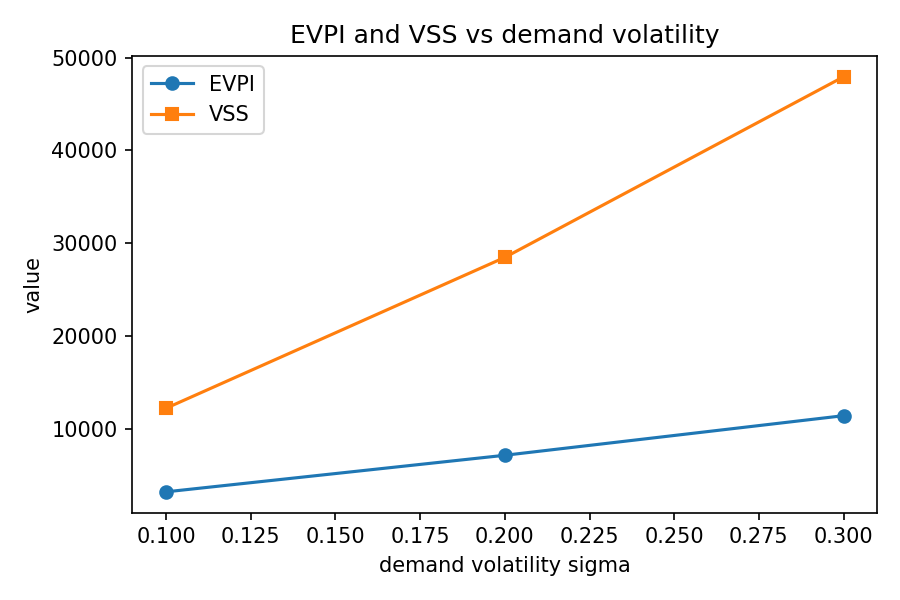
\includegraphics[width=0.6\linewidth]{figures/sigma_sweep.png}
  \caption{EVPI and VSS versus demand volatility $\sigma$.}
  \label{fig:sigma}
\end{figure}

\begin{table}[t]
  \centering
  \caption{Effect of the chance-constraint risk level $\gamma$.}
  \label{tab:gamma}
  \begin{tabular}{lrr}
    \toprule
    $\gamma$ & Objective & Expected unmet demand \\
    \midrule
    0.0 & 250954 & 0.00 \\
    0.1 & 238220 & 0.109 \\
    0.2 & 238220 & 0.109 \\
    0.3 & 238220 & 0.109 \\
    \bottomrule
  \end{tabular}
\end{table}

Figure~\ref{fig:map} shows the open facilities for a representative solution, and
Figure~\ref{fig:conv} the Benders lower and upper bounds across iterations of the
classic loop.

\begin{figure}[t]
  \centering
  \begin{minipage}{0.48\linewidth}
    \centering
    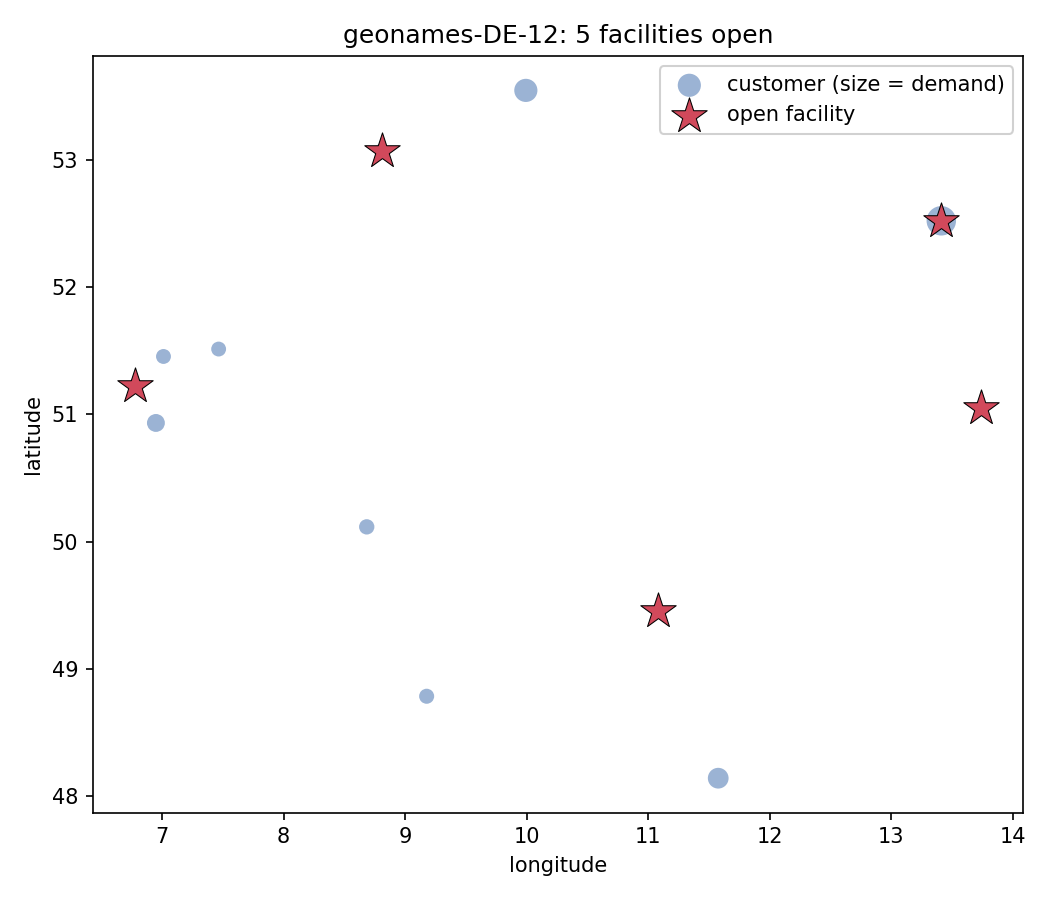
\includegraphics[width=\linewidth]{figures/facility_map.png}
    \caption{Open facilities (stars) and customers (sized by demand).}
    \label{fig:map}
  \end{minipage}\hfill
  \begin{minipage}{0.48\linewidth}
    \centering
    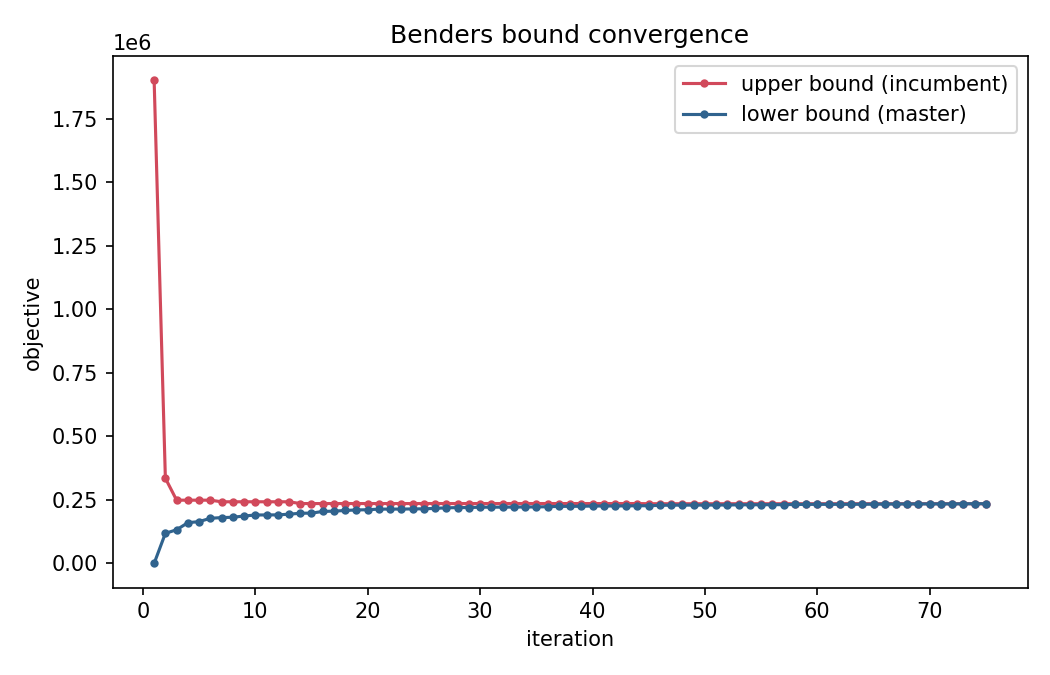
\includegraphics[width=\linewidth]{figures/convergence.png}
    \caption{Benders bound convergence (classic loop).}
    \label{fig:conv}
  \end{minipage}
\end{figure}

\section{Discussion and limitations}
\label{sec:discussion}

The implementation prioritizes correctness, clarity, and solver independence. Its
main limitation is scale. The cut-separation routine is plain Python and solves one
recourse LP per scenario at every candidate first stage; the number of candidates
grows quickly with the number of facilities, and the per-candidate cost grows with
the number of scenarios. As a consequence, instances of roughly twenty facilities
are solved to optimality in seconds to a few minutes, and instances of a few dozen
facilities return a bounded-gap solution within a time limit, but instances of one
hundred or more facilities are beyond what the current routine solves quickly. This
limit is a property of the separation implementation, not of the model or of the
commercial solver: the Gurobi backend exhibits the same behavior because it invokes
the same Python routine at each integer solution.

\section{Conclusion and future work}
\label{sec:conclusion}

We have described a validated, reproducible solver for the two-stage stochastic
CFLP with a service-level chance constraint, solved by SAA and an L-shaped Benders
decomposition with Pareto-optimal cuts and three interchangeable backends. The
solver reproduces published OR-Library optima and the independent monolithic
objective, and it quantifies the value of the stochastic solution and of perfect
information on instances built from real data. The clear next step is to remove the
separation bottleneck---by batching or vectorizing the scenario subproblems, or by
solving them in a compiled routine---which would extend the approach to the
hundred-node instances that the formulation and the commercial backend can in
principle handle.

\paragraph{Reproducibility.}
The source, configurations, tests, and the script that produces every number and
figure in this report are available in the project repository. Each run records its
seed, package and solver versions, and git commit.

\bibliographystyle{plainnat}
\bibliography{references}

\end{document}
